\documentclass[a4paper]{article}
\usepackage[utf8]{inputenc}
\usepackage{amsmath}
\usepackage{amssymb}
\usepackage{caption}
\usepackage{mathtools}
\usepackage{amsfonts}
\usepackage{lastpage}
\usepackage{tikz}
\usepackage{float}
\usepackage{placeins}
\usepackage{textcomp}
\usetikzlibrary{patterns}
\usepackage{pdfpages}
\usepackage{gauss}
\usepackage{fancyvrb}
\usepackage[table]{colortbl}
\usepackage{fancyhdr}
\usepackage{graphicx}
\usepackage[margin=2.5 cm]{geometry}

\definecolor{listinggray}{gray}{0.9}
\usepackage{listings}
\lstset{
	language=,
	literate=
		{æ}{{\ae}}1
		{ø}{{\o}}1
		{å}{{\aa}}1
		{Æ}{{\AE}}1
		{Ø}{{\O}}1
		{Å}{{\AA}}1,
	backgroundcolor=\color{listinggray},
	tabsize=3,
	rulecolor=,
	basicstyle=\scriptsize,
	upquote=true,
	aboveskip={0.2\baselineskip},
	columns=fixed,
	showstringspaces=false,
	extendedchars=true,
	breaklines=true,
	prebreak =\raisebox{0ex}[0ex][0ex]{\ensuremath{\hookleftarrow}},
	frame=single,
	showtabs=false,
	showspaces=false,
	showlines=true,
	showstringspaces=false,
	identifierstyle=\ttfamily,
	keywordstyle=\color[rgb]{0,0,1},
	commentstyle=\color[rgb]{0.133,0.545,0.133},
	stringstyle=\color[rgb]{0.627,0.126,0.941},
  moredelim=**[is][\color{blue}]{@}{@},
}

\lstdefinestyle{base}{
  emptylines=1,
  breaklines=true,
  basicstyle=\ttfamily\color{black},
}

\pagestyle{fancy}
\def\checkmark{\tikz\fill[scale=0.4](0,.35) -- (.25,0) -- (1,.7) -- (.25,.15) -- cycle;}
\newcommand*\circled[1]{\tikz[baseline=(char.base)]{
            \node[shape=circle,draw,inner sep=2pt] (char) {#1};}}
\newcommand*\squared[1]{%
  \tikz[baseline=(R.base)]\node[draw,rectangle,inner sep=0.5pt](R) {#1};\!}
\newcommand{\comment}[1]{%
  \text{\phantom{(#1)}} \tag{#1}}
\newcommand{\pd}[2]{%
  \frac{\partial^{#2}}{\partial #1^{#2}}}
\def\el{[\![}
\def\er{]\!]}
\def\dpip{|\!|}
\def\MeanN{\frac{1}{N}\sum^N_{n=1}}
\cfoot{Page \thepage\ of \pageref{LastPage}}
\DeclareGraphicsExtensions{.pdf,.png,.jpg}
\author{Nikolaj Dybdahl Rathcke (rfq695) \\
        Victor Petren Bach Hansen (grn762) \\
        Tobias Hallundbæk Petersen (xtv657) }
\title{Signal and Image Processing \\ Assignment 5}
\lhead{SIP}
\rhead{Assignment 5}

\begin{document}
\maketitle

\section*{Question 1}
The definition of the Radon transform $p$, which transforms a given distribution $f(x,y)$ into what often is refered to as a \textit{sinogram}, is given by:
$$
  p(\xi, \phi) = \int \int f(x,y) \delta (x\cos \phi + i\sin \phi - \xi)dx\: dy
$$
Figure \ref{1a} shows the provided images \texttt{box.png}, \texttt{sinogram.png} and a non-central point source image.
\begin{figure}[H]
  \centering
  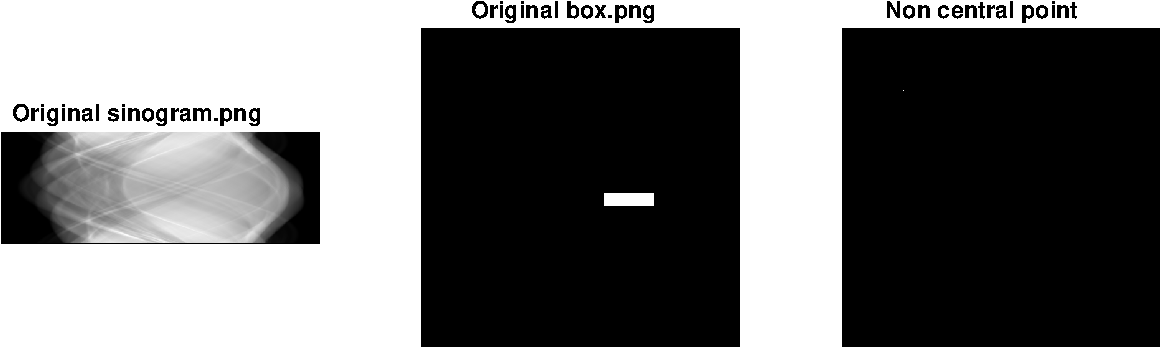
\includegraphics[width=0.8\textwidth]{./1a.pdf}
  \caption{The original images handed out for the assignment, along with 256x256 image with a non centered point at (50,50)}
  \label{1a}
\end{figure}
The implemented radon transform function computes the line integrals from multiple sources (1 for each pixel row) along parallel paths, or beams, in a certain direction. To represent an image, the implemented function takes multiple, parallel-beam projections of the image from different angles by rotating the source around the center of the image and summing each row.
\begin{figure}[H]
  \centering
  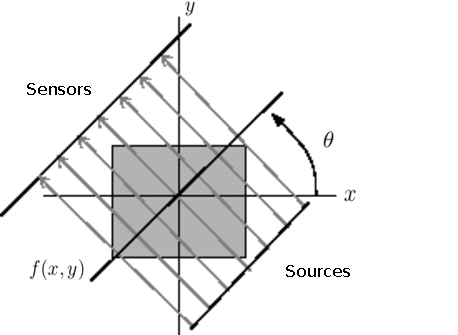
\includegraphics[width=0.8\textwidth]{./1c.pdf}
  \caption[Caption for LOF]%
    {Single parallel-beam projection at rotation angle $\theta$ (Figure kindly borrowed, and sligthly modified, from the Mathworks website: http://se.mathworks.com/help/images/transform74.gif)}
  \label{1c}
\end{figure}
Applying the Radon transform on \texttt{box.png} and the non-central point source image, can be seen below in Figure \ref{1b}:
\begin{figure}[H]
  \centering
  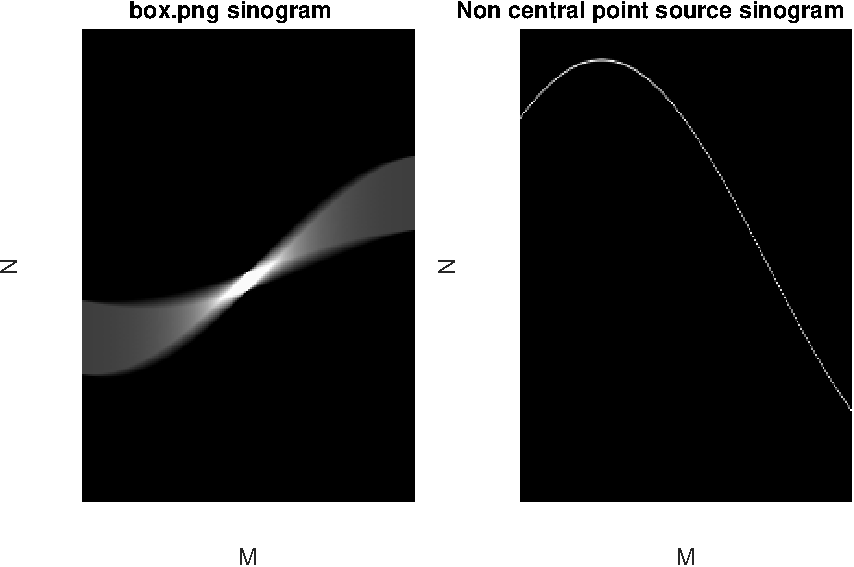
\includegraphics[width=0.8\textwidth]{./1b.pdf}
  \caption{Sinogram for \texttt{box.png} as well as a sinogram for an image of a non-centered point.}
  \label{1b}
\end{figure}
We can from Figure \ref{1b} see that the Radon transform of a small object appears graphically as a number of blurred sine waves with different amplitudes and phases, or in the case of the non-central point source, a single sinosodial wave.
\FloatBarrier

\section*{Question 2}
Backprojection is the idea of taking a Radon transform of an image, the sinogram, and propagate it back into the image space along the projection paths. This operation was performed on the sinogram of the image \texttt{box.png} and a non-central point source that were generated in question $1$, as well as the image \texttt{sinogram.png}. \\
These were generated using the Fourier Slice Theorem, which states that a $1$-dimensional Fourier transform of a sinogram is equal to the $2$-dimensional Fourier transform. Thus, we can simply just take the inverse Fourier transform of the produced $2$ image to reconstruct the original image. The result from doing so is seen in Figure \ref{2}.
\begin{figure}[H]
  \centering
  \captionsetup{justification=centering}
  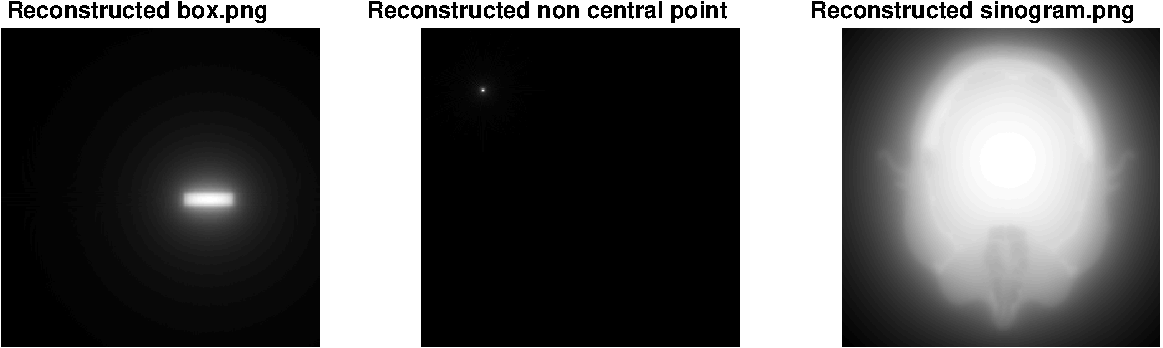
\includegraphics[width=0.8\textwidth]{./2.pdf}
  \caption{Filtered recontruction from sinograms using backprojection, using $M=180$.}
  \label{2}
\end{figure}
The effect we see is the reconstruction are much brighter and a little blurrier. This is due to an overlapping between the Fourier transformed images around the low frequency region. The effects can, however, be controlled if we use a filter in the reconstruction phase.

\FloatBarrier

\section*{Question 3}
As the previous question sets the stage for, we want to produce the reconstructions using a filter. The filter we use is called the ramp filter. This filter does not permit low frequencies, but it will pass high frequencies. This results in an image with less blur and pixels with high contrasts are made more noticeable. The filter is applied by multiplying it to the image in the Fourier domain. Running the same procedure as before, but using the filter, will generate the images seen in Figure \ref{3}.
\begin{figure}[H]
  \centering
  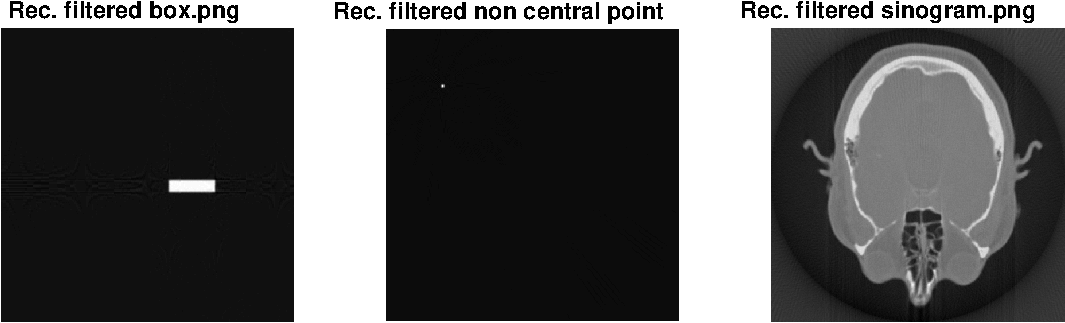
\includegraphics[width=0.8\textwidth]{./3.pdf}
  \caption{Reconstruction from sinograms using backprojection, using $M=180$.}
  \label{3}
\end{figure}
As we can see, the images are much more "normal" in the sense they are less bright and less blurry than those generated without a filter. This is becase the filter accentuates the high-contrasting features, while minimizing the blurring of the image.

\FloatBarrier

\section*{Question 4}
Below in Figure \ref{4b} and \ref{4c} two experiments have been caried out, showing the effect of using different values for $M$ for the sinogram of \texttt{box.png} (also with varying $M$, the same as used for reconstruction) and \texttt{sinogram.png}, when performing the filtered inverse Radon transform.
\begin{figure}[H]
  \centering
  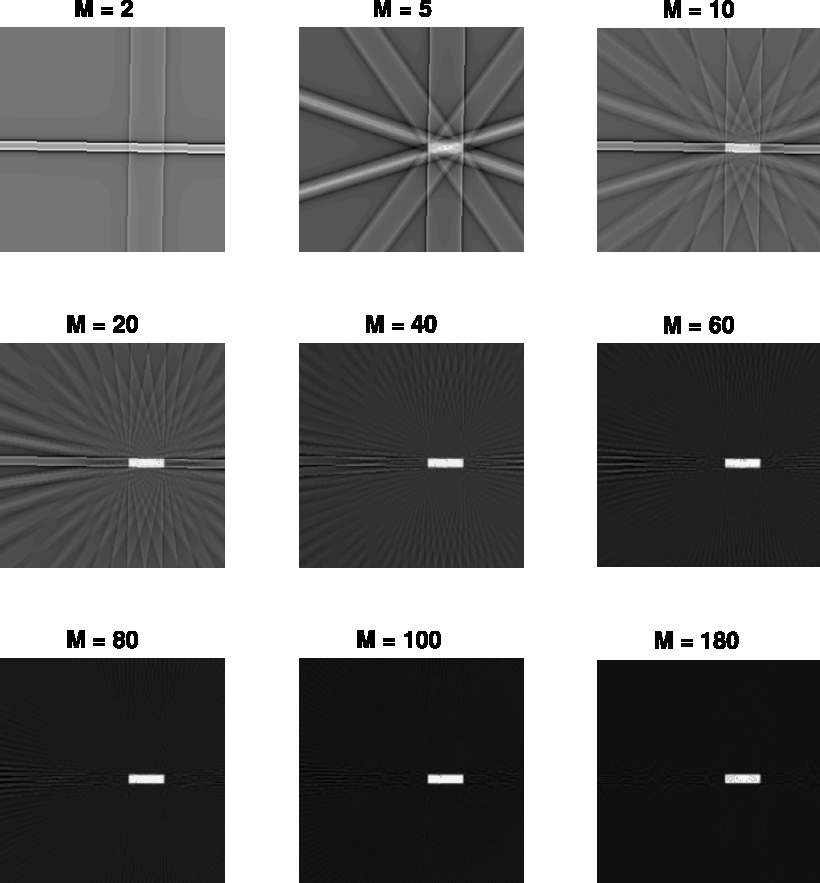
\includegraphics[width=0.8\textwidth]{./4b.pdf}
  \caption{Filtered reconstruction from sinograms of \texttt{box.png} using backprojection. With $M \in \{2,5,10,20,40,60,80,100,180\}$}
  \label{4b}
\end{figure}
Looking at Figure \ref{4b} we can see that increasing $M$ grants a better reconstruction, this makes perfect sense as more projections are added, the quality of the reconstruction will increase, as there is more information to reconstruct the image from. When $M$ is relatively low (around $1$ to $20$), the image contains quite alot of artifacts in the backproject, but as the original image is a very simple one, you can easily make out what it is supposed to be. You can also notice that when
$M=100$, we start to gain very little improvement by adding additional projection, when comparing it to $M=180$.
\begin{figure}[H]
  \centering
  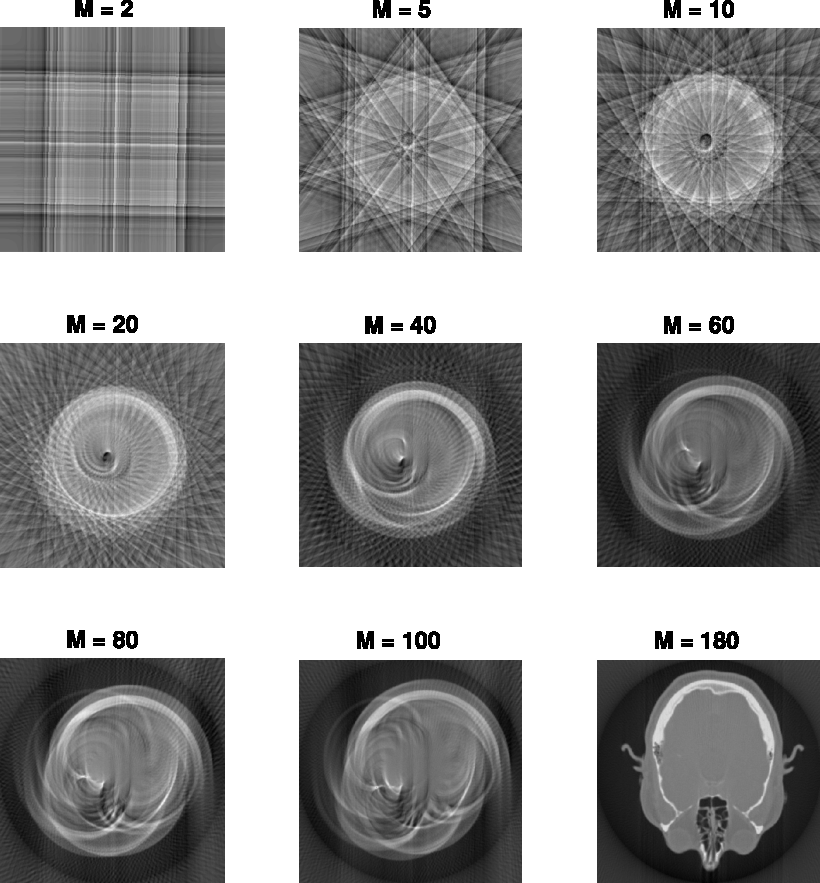
\includegraphics[width=0.8\textwidth]{./4c.pdf}
  \caption{Filtered reconstruction from \texttt{sinogram.png} using backprojection. With $M \in \{2,5,10,20,40,60,80,100,180\}$}
  \label{4c}
\end{figure}
Looking at Figure \ref{4c} we can conclude mostly the same as with Figure \ref{4b}, i.e. more projections means a more accurate reconstruction, and that the image for low values of $M$ contain many artifacts.

However, as the reconstructed image is a fairly detailed one, when using $M=100$ projections, it is still hard to see what the reconstructed image is supposed to look like, when comparing it to the more accurate reconstruction using $M=180$. So we can conclude that we can get away with using fewer projections when the image is less detailed, than the very detailed ones.
\end{document}
